\chapter{Observing Brownian Motion at a Microscopic Scale}
\thispagestyle{fancy}
\fancyhead[RE,LO]{Experiment \thechapter}
%
So far in the laboratories, we have been exploring motion of objects traveling in one particular direction.
We were able to connect this motion to forces because, in the cases we analyzed, the sum of the forces applied to the objects did not change significantly from frame to frame.
This allowed us to apply Newton's laws and connect forces and observed motion.
The objects we studied underwent what we call directed motion.
\par
In contrast, for small objects inside a fluid, the pushes and pulls from the surrounding fluid change very rapidly, and thus the sum of the applied forces is changing magnitude and direction much faster than the fastest imaging frame rate (i.e., faster than our cameras can capture).
On average, when the object is pushed to the right in one frame it will be pushed to the left in another frame.
So, when looking at such small objects with our camera we no longer see directed motion, we see random motion.
Such random motion is experienced by all microscopic objects and is an important attribute for living systems: cells — and the molecules, proteins, DNA and lipids within them — are always in seemingly chaotic motion, so it is essential to understand and characterize this volatile behavior if we hope to make sense of the biological world!!
\par
For the remainder of the semester, you will have the chance to explore many aspects of random motion.
During this three-week lab you will characterize some essential features of random motion and explore the dependence of random motion on particular experimental parameters.
Following this lab, you will investigate motion that is random and directed at the same time (Lab 4) and then consider the analysis of intracellular motion in a living system, including the connections of this motion to work and energy (Lab 5).
\par 
The broad structure of this experiment is provided to you so that the smaller investigations piece together to give a unified picture of random motion and diffusion — but MANY decisions still need to be made by you in order for you to gather and interpret the data.
You should be careful and thoughtful as you create and record your experimental protocol!
Since random motion is most easily measured for microscopic systems, we will be exploring it by studying the motion of microscopic beads in fluid under a microscope.
\par
Since the motion looks different for each bead, if we want to make statements about the group it will be crucial to measure the motion of many beads (say 15-20).
It will be useful for you to measure averages over all beads, but also to create histograms to see the variability from bead to bead (just like you might be curious to know both the average grade and histogram of grades in an exam).
When working with histograms, it will be necessary to track EVEN MORE beads (say 40-50), so that there are sufficient representatives in each `bin' of the histogram.

\paragraph{For this three week lab:} Your overall task for the next three weeks is to characterize the random motion of beads suspended in fluid and determine how the variation of experimental parameters (such as bead mass and size, and the fluid viscosity) impacts the movement of the beads and their resulting diffusion.
You will do this in multiple stages:
\begin{enumerate}
\item Make sure you understand how to safely operate the microscope, how to capture video with the microscope, and the pixel-to-distance ratio of the microscope camera.
\item Capture your first videos and do a preliminary analysis
\item Discuss as a class the method you plan to use to analyze your videos.
\item Collect three videos according to Table \ref{tab:exp3video}.
\item Analyze all of your videos according to the class plan to characterize the behavior of the random motion.
\item Discuss as a class if you need to do any further analysis. Once complete, distribute the data to all groups.
\item Analyze all the data to determine how the variation of parameters affects diffusion.
\end{enumerate}

\section{Exploratory Analysis of Random Motion}
Begin by making sure that you know how to use the microscope.
Make sure the stage is level by using the shims available in the lab.
To get a sense for scale, start by taking a look at the calibration images, located in a file on the desktop.
These will allow you to determine the pixel-scale of your image.
Next, use the microspheres which have been dried to a glass slide to properly adjust the focus and illumination of the microscope.
\paragraph*{Gather your first videos} 
Table \ref{tab:exp3video} has a summary of the the parameters that are being investigated by each group.
Check with your TA if you are unsure of your group number.
Here are some helpful hints:
\begin{enumerate}
\item As you prepare each slide, remember to shake the vial of solution before you extract a sample with the pipette. Your video should be collected fairly quickly after the sample is deposited on the slide. If it takes too much time (e.g., more than 10 minutes), you may want to make another preparation of the sample.
\item Use the 40X objective for these bead videos.
\item Capture 2 videos to get a good overview of random motion before you complete your full analysis:
\begin{itemize}
	\item Capture around 5 seconds of video at 30 fps.
	\item Capture a `low fps' video (see the Microscope Basics Technical Document) at 1 fps for 30 seconds. 
\end{itemize}
\item Be sure to RECORD the video resolution and frame rate for EACH video as soon as you have captured the video. (Usually this is done in the file name itself, by naming your videos something like `2umSilica-H20-40x1280-30fps-001.avi' or `2umPS-lowGly-40x1280-1fps-001.avi')
\end{enumerate}
\paragraph*{Harvest the data out of the video files.}
\emph{Note: Do not set the scale of your video, Multitracker will not work if you do that.}
\begin{enumerate}
\item Open your video file in ImageJ. In the `AVI Reader' window that opened before the video loads, check `Convert to Grayscale' and uncheck `Use Virtual Stack'.
\item We need to threshold the video so that the microspheres are black on a white background. Navigate to `Image $>$ Adjust $>$ Threshold' and adjust the sliders until only the microspheres are black. Depending on the shading and focusing of your initial video, sometimes only the centers of the microspheres will be black. This will still work, as we only need to track the motion of the center of the microspheres (and because you are able to calculate the pixel-scaling from the calibration images).
\item After properly setting your threshold limits, click `Apply'. In the `Convert Stack to Binary' window that opens, uncheck `Calculate threshold for each image' and click OK. Close the Threshold window.
\item Zoom in on one of the particles and use the *Oval* tool to measure its area. You'll use this number as a guide for setting the particle size lower limit of the automatic tracker.
\item Open the `MultiTracker' plugin. Enter a `Minimum Object Size' below the size of your particles to avoid tracking stray noise (usually about half of the area that you measured in the previous step works well). Check the boxes next to `Show Lables', `Show Positions', and `Show Paths'. Click OK.
\item After running through its calculations, the plugin should have done the following things (see figure \ref{fig:multitracker} for an example):
\begin{itemize}
	\item All the particles in the video now have a label with a number assigned to them by the plugin and their position.
	\item A window `Path' opens that shows the motions of the tracked particles throughout the video. (Though this may not necessarily be useful in your analysis, it does give you a way of quickly checking your data. For instance, in the example data in figure \ref{fig:multitracker}, what common feature of the paths point to a problem with the setup when that data was captured?)
	\item A results window opens that displays the X and Y position of each particle in each frame.
\end{itemize}
\item Copy and past the results into excel.
\item Watch the video and delete the data of any spheres that leave the image or seem to encounter some other type of problem.
\end{enumerate}
\begin{figure}[ht]
	\centering
	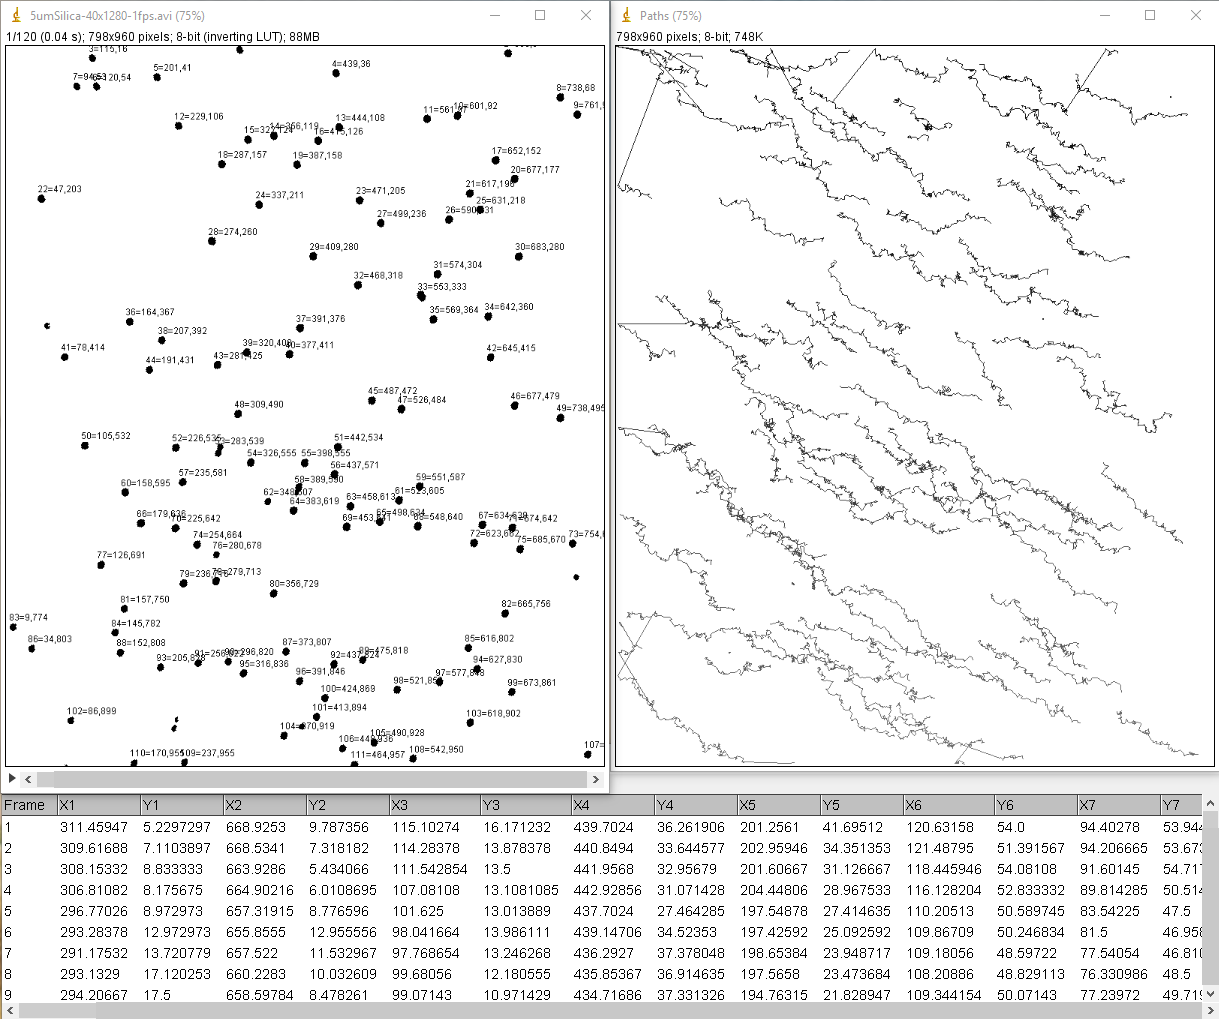
\includegraphics[width=\linewidth]{multitracker}
	\caption{Example Multitracker analysis of microsphere motion}
	\label{fig:multitracker}
\end{figure}

\paragraph*{Characterize the random motion of the beads in your videos.} Compare and contrast their motion to what you would expect for directed motion.
\begin{itemize}
\item Do the average total $x-$ and $y-$ displacements of the beads, $\left \langle \Delta x \right \rangle$ and $\left \langle \Delta y \right \rangle$, change throughout the time intervals you observed? If so, how do they change; if not, why don't they change?
%\item How do the individual total $x-$ and $y-$ displacements of the beads, $\Delta x$ and $\Delta y$, change throughout the time intervals you observed? [\textit{Hint: Make some histograms!}] If so, how do they change; if not, why don't they change? How are these individual displacements linked to the average displacements?
\item How does the total displacement of a particle, $r=\sqrt{\Delta x^2+\Delta y^2}$ , change as a function of the measurement time interval?
\end{itemize}

\begin{table}[ht]
\centering
\begin{tabular}{|p{4.5cm}|p{3cm}|p{3cm}|p{3cm}|}
\hline
 \textbf{Group \# (Parameter)} & \textbf{Video 1} & \textbf{Video 2} & \textbf{Video 3}  \\
 (each parameter will be investigated by two distinct groups, allowing you to `double check' the results) & (condition for testing r$^2$ vs.\ t dependence) &  & \\ \hline
 \textbf{1 \& 2 (bead size)} & 2 $\mu$m silica beads in water & 5 $\mu$m silica beads in water & 1 $\mu$m silica beads in water \\ \hline
 \textbf{3 \& 4 (fluid viscosity)} & 2 $\mu$m silica beads in water & 2 $\mu$m silica beads in low viscosity glycerin/water mix & 2 $\mu$m silica beads in high viscosity glycerin/water mix \\ \hline
 \textbf{5, 6, \& 7 (bead mass \& viscosity)} & 2 $\mu$m PS beads in water & 2 $\mu$m PS beads in low viscosity glycerin/water mix & 2 $\mu$m PS beads in high viscosity glycerin/water mix \\ \hline
\end{tabular}
\caption{Video Summary}
\label{tab:exp3video}
\end{table}

\paragraph*{Plan your analysis.} Use the `Leading a discussion' time to determine, as a class, the best way to analyze your data that allows you to characterizing diffusion.
At the end of the second day of the experiment,  everyone will distribute their data to the rest of the class.
Therefore, make sure that your data files are easy to follow, and that your graphs look professional.

%Day 2
\section{Measuring \& Analyzing Random Motion}
At the end of the first day of this experiment, during the post-experiment discussion, your TA provided you with some information about the Diffusion Constant. 
Begin your second day of this experiment by completing your analysis of video 1 using the plan that you decided as a class would be the best way to characterize diffusion.
Then capture and analyze videos 2 and 3.
\begin{enumerate}
\item \textbf{Examining Diffusion for Video 1:} Does the diffusion constant, D, depend on the measurement time interval (i.e., is D frame rate-dependent)? Using the information you have already created for your first video, investigate how the square of the average bead displacement, $r^{2}$, changes for different measurement time intervals, $\Delta t$. What is the diffusion constant for your video 1?
\item \textbf{Collecting Data for Videos 2 and 3:} These videos have been carefully chosen so that the class, as a whole, can make statements about how varying specific parameters affects the diffusion constant. The parameters of the videos that you capture (i.e., the frame rate, resolution, length, etc.) should be based on what you decided to do as a class at the end of the first day. 
\item \textbf{Analyzing Videos 2 and 3:} Analyzing this data will allow you to combine your results with other groups' work and make claims about how varying the investigated parameter affects the diffusion constant. As with video 1, you will want to analyze these videos according to the plan you came up with as a class. Make a back-up of your data before you begin. Also, make a plan for how to manipulate your data BEFORE you do any calculations in your spreadsheet. (Planning now saves time later!)
\item \textbf{Coordinate with fellow groups.} If you measured the same parameters as another group, meet with them and combine your data before it is sent to the other groups.
\end{enumerate}

\paragraph*{Review your analysis.} Use the `Leading a discussion' time to determine, as a class, if the methods you decided on at the end of the first day are properly characterizing diffusion. If any changes need to be made, work to re-do the analysis before the end of this class. 

%Day 3
\section{Characterizing Random Motion and the Diffusion Constant}
Over the last two weeks, you fully characterized the random motion of beads in fluid and began to determine how changing one parameters of the solution (beads in fluid) can affect the diffusion constant.
In this final week of the lab, you will combine your results with those from the rest of the class, and determine how other parameters of the bead solutions will affect the diffusion constant.
\emph{The data collected by all groups should be included in your lab report.}

\begin{enumerate}
\item \textbf{Examine Diffusion:} Using the data that all of the lab groups have collected over the course of this lab, you are expected to make an argument for a plausible expression for the diffusion constant, D, as a function of some (or all) of the following parameters: fluid viscosity, bead size, and bead mass. (An argument should contain a Claim, Data, and a Warrant—i.e., an explanation of how the claim is related to the data.) You should confirm that this mathematical model for D is plausible by performing a dimensional analysis.
\item \textbf{Things to consider including in your lab report:} As you know, what goes into your lab report should be determined by the ideas necessary to explain and support your work—in designing the experimental protocol, in collecting and analyzing your data, and in forming your conclusions. Here are a few questions you might consider answering:
\begin{itemize}
\item What characteristics have you observed for random motion? (How would these characteristics be similar or different for directed motion?)
\item If the average total displacement in either the x- or the y-direction is zero for all times, why is the displacement NOT zero? How does the displacement change with time?
\item What is the mathematical model that you have constructed for the diffusion constant, D? How is this justified by your experimental data? Do the dimensions work out?
\item How could we design an experiment to find the exact form for the diffusion constant (i.e., how could we figure out the numerical constants that accompany the scaling of D with bead mass, bead radius, viscosity, and temperature)?
\item What could you have done better in your own design and analysis?
\item How are these ideas of random motion and diffusion constants related to (important in) other scientific disciplines?
\end{itemize}
\end{enumerate}

%\subsection*{Equipment}
%Familiarize yourself with the Microscope Basics Technical Document before beginning any experimentation. 
%If you do not know how a particular part of the microscope works, please ask your TA — the equipment is expensive! 
%Please be especially careful handling liquid samples near the microscope objectives. 
%\par
%The CCD camera attached to the microscope will allow us to capture video of what we observe. 
%Using the same VirtualDub software we utilized in previous weeks, we can capture AVI videos of the motion we are trying to analyze. 
%In VirtualDub, the microscope camera can be found under `Device' and is named ``ToupCam (DirectShow)''. 
%\par  
%The adjustment options for the microscope CCD camera are slightly less user friendly than the webcam options. 
%However, they are still found in the same VirtualDub menus. 
%Be sure to take note of at which resolution you record your videos; it will be important when determining the distance to pixel ratio. 
%This can be done by taking a picture of the 1 mm calibration slide at the same resolution and magnification level as your videos. 
%If calibration slides are not available, pictures can be found on the lab computers. 
%\par 
%Brightness, contrast, and other exposure settings can be found under `Video' and `Capture Filter'. 
%The most important difference from the webcam cameras is that the frame rate cannot be directly set before capturing videos. 
%It is necessary to control the frame rate by controlling the exposure time of the CCD camera. 
%By telling it to expose the CCD to light for 100 ms intervals, for instance, you are telling it to take a picture every 0.1 seconds.
%This also means that you have to carefully control the amount of light through your sample using the iris and bulb power control. 
%If you are having trouble getting the light settings correct, you can use the Auto Exposure option, but this will often result in very low frame rates.
%
%Since all three videos have captured random motion, we need only look at one video to begin characterizing the behavior of random motion. 
%(Also, you may learn tricks and ideas that can help you analyze the other videos in the coming weeks. Next week, we will teach you automatic tracking!) 
%The method you use to harvest the data is a bit different from what you have done previously with ImageJ. 
%Rather than tracking each object of interest through EVERY frame of the video, we can take very specific frames (reducing the number of clicks you need to make). 
%So, for the beads that you are tracking, you want an initial position (at t=0, the first frame), a final position (at the last frame), and at least 4 other positions (at specific frames equally spaced between the initial and final frame). 
%This will take some careful planning once you have the video in ImageJ and BEFORE you open the Manual Tracking plugin. 
%To compare these beads with each other (histogram-style), you need to be tracking these beads in the all of the SAME frames. 
%For the first video ONLY, we suggest 40-50 beads should be tracked (so that you can create good histograms). 
%For videos 2 and 3, you can use only 15-20 beads (which should be sufficient for the RMS analysis).
%
%On the final day of class, your group will compile all of this data in your lab report as you discuss the effects that these parameters have on the random motion of particles.
%
%\item \textbf{Give Presentations:} Before finishing your lab reports, you should present your work to your peers for critical evaluation. Being part of a community of scientists means sharing your work (in professional journals, through symposia, and at conference talks and poster sessions) for critical evaluation and revision by the community. To model this important aspect of scientific practice, you will create posters presenting your methods, findings, and conclusions. Highlight the important features of your work, your analysis, and your results. During the presentations, ask other groups about what they have done and do not be afraid to ask challenging questions. Your goal is to understand what they have done and how they can improve their work. When you present your work to them, they should ask the same types of challenging questions of you and your group. This should spark some interesting discussions that you can incorporate into your lab report in the evaluation/critic's section.
%
%This week you will continue to explore this random motion, finalizing your histograms ($\Delta$x, $\Delta$y, and r) at various times for video 1 (2 micron beads in water). 
%When your histograms are finished and you have answered the questions asked in last week's lab document (repeated below), fully characterizing the nature of random motion, you should begin analyzing videos 2 and 3. 
%In order to do this, it might help to have a little more information. 
%\par 
%You will discover, as you build your total RMS displacement histograms, that the average displacement magnitude, i.e.\ the average distance traveled by the beads (let’s call it $\left< r \right>$), deviates from zero: Every bead changes its position by some amount! 
%As you remember, the distance traveled can be calculated as $r = \sqrt{\Delta x^{2}+\Delta y^{2}}$, including only the squares of $\Delta$x and $\Delta$y — which are always positive and so add up to something bigger than zero. 
%This equation indicates that instead of the distance traveled, r, we can measure the square of the distance traveled $r^{2} = \Delta x^{2} + \Delta y^{2}$, also called the Mean Squared Displacement or MSD. 
%This makes the math a bit easier, and r$^{2}$ increases linearly with the measurement time interval, as you will see today. 
%\par 
%The ``diffusion constant,'' D, is defined to be the proportionality constant between the average displacement squared, $r^{2}$, of the diffusing object and the measurement time interval, $\Delta$t, over which the diffusion occurs. 
%There is also a factor of 4 in there (for geometry reasons—a 4 in 2-dimensions, a 6 in 3-dimensions, a 2 in 1-dimension):
%\begin{equation}
%r^{2} = 4 D \Delta t
%\end{equation} 
%
%Table
%\begin{tabular}[bt]{|p{.3\textwidth}|p{.2\textwidth}|p{.2\textwidth}|p{.2\textwidth}|}
%	\hline
%	\textbf{Group \# (Parameter)} & \textbf{Video 1} & \textbf{Video 2} & \textbf{Video 3} \\
%	(each parameter will be investigated by two distinct groups, allowing you to `double check' the results) & (condition for testing r$^2$ vs.\ t dependence) &  &\\
%	\hline
%	1 \& 4 (bead size) & 2 $\mu$m silica beads in water & 5 $\mu$m silica beads in water & 1 $\mu$m silica beads in water \\
%	\hline
%	2 \& 5 (fluid viscosity) & 2 $\mu$m silica beads in water & 2 $\mu$m silica beads in low viscosity glycerol/water mix & 2 $\mu$m silica beads in high viscosity glycerol/water mix \\
%	\hline
%	3 \& 6 (bead mass \& viscosity) & 2 $\mu$m PS beads in water & 2 $\mu$m PS beads in low viscosity glycerol/water mix & 2 $\mu$m PS beads in high viscosity glycerol/water mix \\
%	\hline
%\end{tabular}